\documentclass[11pt, oneside]{article} %Use "amsart" instead of "article" for AMSLaTeX format

\usepackage[left=2cm,top=3cm,right=2cm,bottom=4cm,head=1cm,a4paper]{geometry}    
\usepackage[utf8]{inputenc}
\usepackage{graphicx} %Use pdf, png, jpg, or eps§ with pdflatex; use eps in DVI mode
\usepackage{graphicx}
\usepackage{amsmath}
\usepackage{amssymb}
\usepackage{hyperref}
\usepackage{soul}
\usepackage{dsfont}
\usepackage{cleveref}

\usepackage{amsmath}
\usepackage{multicol}
\usepackage{amssymb}
\setlength\intextsep{11pt}
\usepackage{braket}
\numberwithin{equation}{section}
\usepackage{bm}
\usepackage{appendix}
\usepackage{microtype}
\usepackage{titlesec}
\usepackage{mathpazo}
\usepackage{titlesec}
\usepackage{hyperref}
\usepackage{subfiles}
\usepackage{bbm}
\hypersetup{
    colorlinks,
    citecolor=black,
    filecolor=black,
    linkcolor=black,
    urlcolor=black
}
\usepackage[
    backend=biber, 
    style=phys,
    citestyle=numeric-comp,
    biblabel=brackets, 
    hyperref=true,
]{biblatex}
\bibliography{refs}

% math commands:
\newtheorem{theorem}{Theorem}

\newcommand*{\vertbar}{\rule[-1ex]{0.5pt}{2.5ex}}
\newcommand*{\horzbar}{\rule[.5ex]{2.5ex}{0.5pt}}
\newcommand{\dline}[1]{\underline{\underline{#1}}}

\newcommand{\tr}{\ensuremath{\textup{Tr}}}
\newcommand{\1}{\ensuremath{\mathbbm{1}}}
\newcommand{\re}{\ensuremath{\textup{Re}}}
\newcommand{\im}{\ensuremath{\textup{Im}}}
\newcommand{\ts}{\textsuperscript}
\renewcommand{\r}{\ensuremath{\textbf{r}}}
\newcommand{\jon} {J_{\textup{on}}}
\newcommand{\joff} {J_{\textup{off}}}
\newcommand{\ketbra}[2]{\ket{#1}\!\bra{#2}}
\newcommand{\qkit}{\mathcal Q_{\textup{Kit}}}
\newcommand{\ujk}{u_{jk}}
\newcommand{\pf}{\textup{pf}\,}
\newcommand{\pdag}{\phantom{\dag}}


\newcommand{\loctr}{\textup{tr}}
\newcommand{\egs}{E_\textup{g.s.}}

\newcommand{\normord}[1]{{\,}^\ast_\ast  #1 {\,}^\ast_\ast}
\renewcommand{\ts}{\textsuperscript}

\newcommand{\peru}[1]{{\color[rgb]{0.4,0.,0.8}[\textbf{Peru:} #1]}}
\newcommand{\justin}[1]{{\color[rgb]{1,0.5,0.}[\textbf{Justin:} #1]}}
\newcommand{\noteAG}[1]{{\color[rgb]{0.,0.4,0.1}[\textbf{Grushbot Decrees:} #1]}}
\newcommand{\addAG}[1]{{\color[rgb]{0.,,0.4,0.1}{#1}}}


%Define that shaded box you like
\usepackage[noframe]{showframe}
\usepackage{framed}
\renewenvironment{shaded}{%
    \everypar={{\setbox0=\lastbox}\everypar{}}
  \def\FrameCommand{\fboxsep=\FrameSep \colorbox{shadecolor}}%
  \MakeFramed{\advance\hsize-\width \FrameRestore\FrameRestore}}%
 {\endMakeFramed}
\definecolor{shadecolor}{gray}{0.9}


\renewcommand{\thefootnote}{\roman{footnote}}

% \crefformat{section}{\S#2#1#3}
% \crefmultiformat{section}{\S\S#2#1#3}{ and~#2#1#3}{, #2#1#3}{, and~#2#1#3}



\usepackage{wrapfig}
\usepackage{caption}


\title{A quick note on Kasteleyn and Probabilities}

\author{Peru d'Ornellas}
% \date{}

\begin{document}

\maketitle

These are just a few notes so I have it written down somewhere exactly why and how the inverse Kasteleyn matrix computes probabilities. It's a remarkably simple and elegant piece of mathematics.  

\section{The Inverse Kasteleyn Matrix}

Let's start by restating Kasteleyn's theorem, which we shall not prove. For a graph $\Lambda$, we may define a Kasteleyn-oriented  skew-adjacency matrix, $K$. Then the number of valid dimerisations is given by 
\begin{align}
    N = |\pf K|.
\end{align}
Now let's look at the inverse Kasteleyn matrix. In order to derive this, we must first state two properties of Pfaffians, which Can both be found on the Wiki page for the Pfaffian. Firstly, we state the recursive definition of a Pfaffian for a general $2n \times 2n$ matrix, expanded along a row indexed with $i$,
\begin{align}
    \pf K = \sum_{j\neq i}^{2n} (-1)^{i+j+1+\theta(i-j)} K_{ij} \pf{K_{\bar {ij}}},
\end{align}
where the matrix $K_{\bar {ij}}$ is the matrix $K$ with rows and columns $i$ and $j$ removed. Taking a derivative with respect to $K_{ij}$, we arrive at the following identity,
\begin{align}\label{eqn:kij_recursive}
    \frac{d}{d{K_{jk}}} \pf K 
    = (-1)^{i+j+1+\theta(i-j)} \pf{K_{\bar {ij}}}.
\end{align}
Next, let us write down a derivative identity for the Pfaffian, for a matrix with some arbitrary parameter $K(x)$
\begin{align} \label{eqn:deriv}
    \frac{1}{\pf K} \frac d {dx} \pf K = \frac 12 \tr \left ( K^{-1} \frac{dK}{dx}\right ).
\end{align}
Now, let us suppose that our derivative is just in the $ij$ element of $K$. In this case, the $K$ derivative on the right-hand side becomes
\begin{align}
    \frac {dK}{dK_{ij}} = \ketbra ij - \ketbra ji
\end{align}
The second term comes from the condition that $K$ must remain antisymmetric. Thus, the expression \ref{eqn:deriv} becomes
\begin{align} \label{eqn:kij_inv}
    \frac{1}{\pf K} \frac d {dK_{ij}} \pf K = K^{-1}_{ji}.
\end{align}
We now insert \cref{eqn:deriv} into \cref{eqn:kij_recursive}, arriving at the following
\begin{align}\label{eqn:kij_in_k}
    K^{-1}_{ji} = \frac{
        (-1)^{i+j+1+\theta(i-j)} 
        \pf{K_{\bar {ij}}}
    } {
        \pf K
    }.
\end{align}
Finally, taking the modulus of both sides, we can get rid of that factor of $-1$ and arrive at the final well-known identity 
\begin{align}
    |K^{-1}_{ji}| = \left | \frac{
        \pf{K_{\bar {ij}}}
    } {
        \pf K
    }\right |.
\end{align}
Now we consult Kasteleyn's theorem and realise that this is a rather remarkable result! If $ij$ represents an edge on our lattice, then we can be sure that $|\pf{K_{\bar {ij}}}|$ counts the total number of dimerisations on the lattice with edge $ij$ removed, whereas the denominator counts the number of dimerisations on the original lattice. Thus, we have calculated the probability that edge $ij$ is a dimer!
\begin{align}
    p(e_{ij}) = |K_{ij}^{-1}|.
\end{align}

\subsection{Working on the Torus}

So far, everything we have done has been in open boundary conditions. Things become a little more complex when one works on the torus. This is because Kasteleyn's theorem looks rather different on the torus due to the presence of topologically non-trivial loops, which wind the torus in the $x$ and $y$ direction. Thus, we must define four Kasteleyn matrices, indexed by $K^{ab}$, with $a,b \in \{0,1\}$. Each of these indexes denotes whether the boundary conditions are periodic or anti-periodic in that respective direction. Equivalently, they denote the flux threaded through these two non-contractible loops. Again, we shall only state Kasteleyn's theorem for this case, which says that
\begin{align}
    N = \frac 12 \left |  \pf K^{00} -\pf K^{01}-\pf K^{10}-\pf K^{11} \right |.
\end{align}
This time, let's start by writing down the formula for the probability of a single edge hosting a dimer,
\begin{align}
    p(e_{ij}) &= \frac{N_{\bar{ij}}}{N} \\ 
    & = \left |
    \frac
    {\omega_{ab}\pf K_{\bar{ij}}^{ab}}
    {\omega_{cd}\pf K^{cd}}
    \right |,
\end{align}
where we use Einstein summation convention and have defined the sign operator as a shorthand for the sign structure of the torus Kasteleyn theorem,
\begin{align}
    \omega_{ab} = \begin{cases}
        & +1 \text{ if}\;a,b=0, \\
        & -1 \text{ otherwise}.
        \end{cases}
\end{align}
Now, we insert \cref{eqn:kij_in_k}, leading to the following expression for the overall probability,
\begin{align}
    p(e_{ij}) = \left |
    \frac
    {
        \omega_{ab}
        {K_{ji}^{ab}}^{-1}
        \pf K^{ab}  
    % (-1)^{i+j+1+\theta(i-j)}
    }
    {
        \omega_{cd}\pf K^{cd}
    }
    \right |,
\end{align}
This is a bit more complex than the expression for the regular probability but still totally manageable.

\section{Some Neat Tricks on a Semi-regular Lattice}
Now suppose we are working on an amorphous graph which still has the following regular structure, something like this:
\begin{center}
    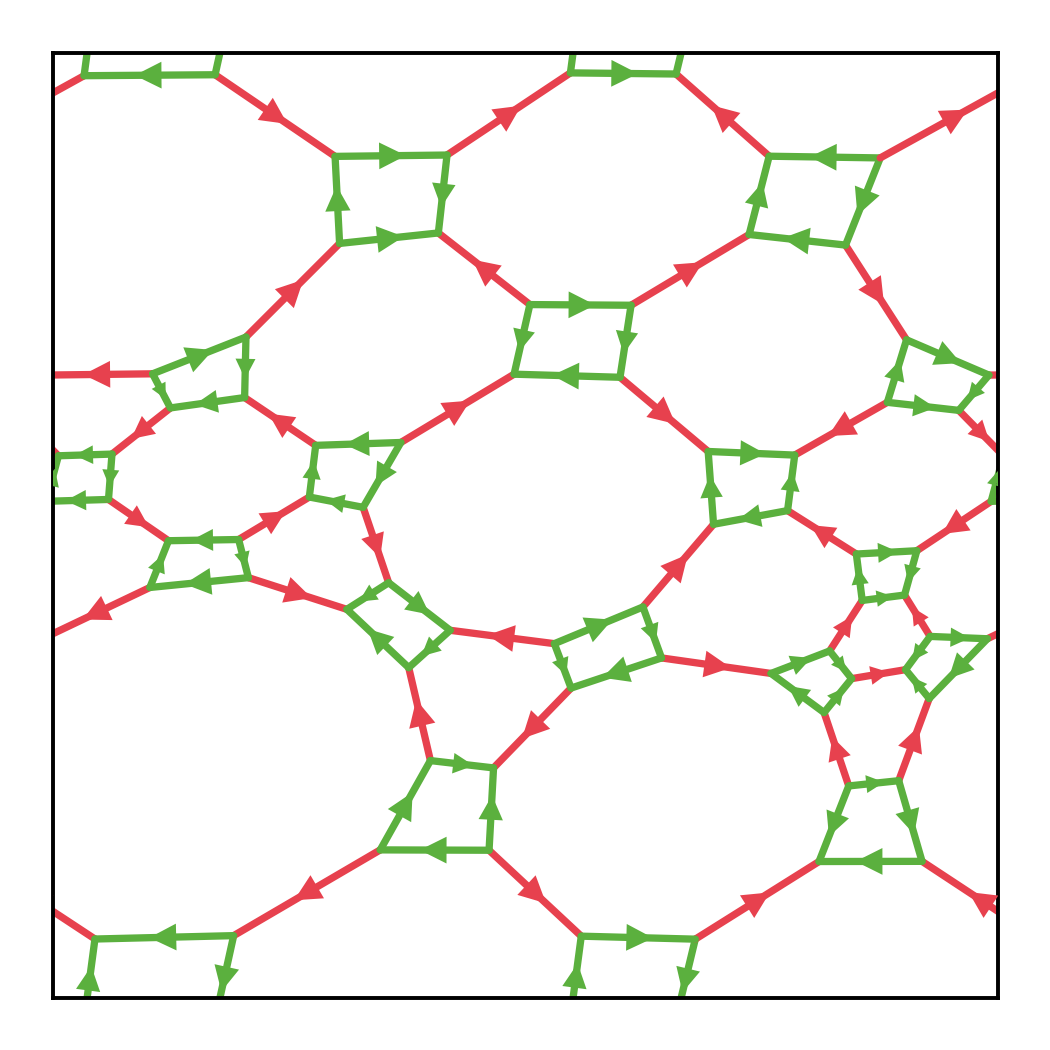
\includegraphics[width=0.3\textwidth]{lattice.png}
\end{center}
where we are represent the Kasteleyn orientation with the arrows, and all loops have an odd number of clockwise arrows. Thus, we can decompose the Kasteleyn `Hamiltonian' into two parts: a term that just lives on each square, $K_{0}$, and a term that connects two squares, $V$, highlighted in green and red respectively,
\begin{align}
    K = u K_{0} + v V,
\end{align}
where $u$ and $v$ parametrise the strength of each bond. Now let us define the resolvent,
\begin{align}
    R(\lambda) = (K-\lambda)^{-1},
\end{align}
which can be decomposed in terms of the `unperturbed' resolvent, $R_0(\lambda) = ( K_0 - \lambda )^{-1},$ using the following series,
\begin{align} \label{eqn:resolvent_expansion}
     R = R_0 + R_0VR_0 + R_0VR_0VR_0 + ...
\end{align}
Obviously, the resolvent is just a fancy word for the matrix inverse which, as we discussed in the previous section, encodes the local dimer probabilities. So basically what we have here is a nice series expansion for the local dimer probabilities. 

Now, let's calculate this expansion. The first thing we want to do is find $R_0$, which is pretty trivial because $H_0$ is just a collection of unconnected squares, where each square has three clockwise arrows and one counterclockwise one\footnote{Or the other way round, but these two configurations are gauge equivalent, just swap all arrows, which is always a gauge transform when we're bipartite.}. Thus, the Hamiltonian $H_0$ is a bunch copies of the following matrix,
\begin{align}
    H_0 \sim h = \begin{pmatrix}
         & 1 &  & 1 \\
        -1 &  & 1 &  \\
         & -1 &  & 1 \\
        -1 &  & -1 &  
    \end{pmatrix}.
\end{align}
This is a rather remarkable operator because it satisfies the property
\begin{align}
    h^2  = -2 \1,
\end{align}
i.e. it is almost idempotent, $h^{-1} = -h/2$. Note that only the square case has this property, the same cannot be said of the hexagonal lattice where we can define an $h_6$ matrix\footnote{More on that later, $h_6$ and $h_8$ still have some lovely properties.}. To find the whole resolvent, let's make an ansatz for the inverse of $\lambda - h$, as the following expression parametrised by $a$ and $b$,
\begin{align}
    \left (
         h- \lambda
    \right )^{-1} = 
        ah + b,
\end{align}
which is satisfied by
\begin{align}
    a = \frac{-1}{2 + \lambda^2}, \\
    b = \frac{-\lambda}{2 + \lambda^2}.
\end{align}
Thus, the resolvent is given by 
\begin{align}
    R_0(\lambda) = \frac{-1}{2+\lambda^2}\left ( 
        h+\lambda 
    \right ).
\end{align}
That was easy! And it's all rather encouraging, since the factor of $1/(2+\lambda^2)$ is going to be rather useful in making sure our infinite sum doesn't blow up!

\subsection{The Resolvent at $\lambda = 0$}

Let's focus on the resolvent at $\lambda = 0$, which is the simplest case, since $R_0(0) = -h/2$.
Now that we have an exact expression for $R_0$, we can start to evaluate the full-system resolvent, $R$, using \cref{eqn:resolvent_expansion}. Specifically, we are interested in calculating the matrix element of $R$ on the bond $(ij)$, which can be written as
\begin{align}
    R_{ij} = -\frac 12 h_{ij} + \frac 14 h_{ i\mu} V_{\mu \nu}h_{ \nu j} -\frac 18 h_{ i\mu} V_{\mu \nu} h_{ \nu\alpha} V_{\alpha \beta}h_{ \beta j} + ...
\end{align}
This is useful because as we have seen, the matrix element of $R(\lambda = 0)$ is precisely the probability of a given site hosting a dimer\footnote{Obviously in periodic boundaries this is complicated slightly, but let's not worry about that for now.}. At each order in the series, the terms can be interpreted as a weighted sum over all paths from $i$ to $j$. 

Naively this looks like it hasn't really helped, path counting is on a disordered lattice is generally pretty hard. However, not all paths are counted in this expression! Our paths have to always be made up of alternating $R$ and $V$ elements, which do different things! Each $R$ step can be viewed as entering and leaving a single green square in the diagram, whereas every $V$ element jumps from one square to the next using a red bond. Furthermore, the $R$ steps only have non-zero matrix elements for two of the four paths across a square, either turning left or turning right, any path that crosses over a square, or hits a square and turns back on itself is forbidden. It turns out that these constraints MASSIVELY reduce the number of paths we need to count in our expansion.

\subsubsection{Counting All Paths}
\subsubsection{The Sign of a Path}



\end{document}

